\section{LAVA Manipulation}

The first step for me was to study in-depth the \gls{lava} software and test to which extent I could use it to help save time for the manual insertion of bugs into production software.

When I arrived at \gls{nist}, the \gls{samate} team was just about to get in touch with the \gls{lava} team. Their project being closely related to our work on improved test material development, we invited them to come at \gls{nist} and organized a meeting so they could introduce to us their work on \gls{lava} software.

This meeting allowed us to realize that both teams were facing similar issues on many matters and that working together could help us solve some of them. For the sake of presenting their automated vulnerability addition framework, they provided us with two \glspl{vm}. Those \glspl{vm} were designed to work together in order to run \gls{lava}.

Getting access to these \glspl{vm} allowed me to get a far-better understanding of how \gls{lava} works. But in order to get them to work, I had to change some configuration settings to make them easier to use, and adapted to my work environment.

\subsection{LAVA VMs Configuration}

The \gls{lava} system is composed of two \glspl{vm} designed to work together. One \gls{vm} is a 64-bit Ubuntu machine, the other is a 32-bit Debian machine. The reason why \gls{lava} needs two \glspl{vm} is that it is experimental software. For some reason, some parts of the \gls{lava} system cannot be executed on 64-bit machines while others need to be executed on 64-bit systems. Using two \glspl{vm} is an undesirable tweak that \gls{lava} developers are actually working on. Not only does this increase the complexity of use of \gls{lava}, but also, it hampers the maintainability of the source code.

\subsubsection{Virtualization Software Compatibility Issues}

I encountered quite a few difficulties trying to set up the \gls{lava} \glspl{vm} on my desktop environment. First of all, I noticed that the provided \glspl{vm} were designed to run on the proprietary virtualization software VMWare \cite{vmware2016official}. Unfortunately, I had no software licence at my disposal. I first asked my division chief if I could get a licence, but the process was too lengthy, up to 1 month to get access to the software. Therefore, I turned myself towards the open source alternative VirtualBox \cite{virtualbox2016official}, knowing that I could face some compatibility problems. Indeed, according to the virtualization software used, the \glspl{vm} format varies, which is sometimes the source of troublesome compatibility issues.

\subsubsection{Network Configuration}

In order to work together, the \gls{lava} \glspl{vm} need to communicate through a network while running the software. This execution is governed by a shared \gls{json} configuration file (Listing \ref{lst:json-config-file}) which contains critical information for the software to run properly. This information includes the relative IP addresses of each \gls{vm} so that the execution flow can bounce from one to an other and be synchronized.

While it was working perfectly out of the box during the \gls{lava} presentation meeting, I simply ran into a bunch of errors, breaking the program and blocking its execution. I realized that the IP addresses given in the \gls{json} configuration file were mistaken. This problem was in fact a consequence of compatibility issues between VMWare and VirtualBox.

Indeed, VMWare and VirtualBox handle the \glspl{vm} network configuration in completely different ways. Whereas VMWare simply assigns dynamically a different IP address to every single \gls{vm} running thanks to a virtual \acrshort{dhcp} (\acrlong{dhcp}) server, VirtualBox keeps the running \glspl{vm} in isolated environments and networks, assigning the same IP address to every \glspl{vm}. This explains why I ended up with errors in the first place.

Moreover, as VMWare keeps assigning the same IP address to each \gls{vm} between different boot times, there were no configuration issues during the \gls{lava} presentation meeting. On the other hand, I realized that VirtualBox behaved differently and was assigning random IP addresses at each boot time. This was a real pain because everytime you would shutdown or restart a \gls{vm}, you would need to modify the configuration file again to specify the right IP addresses.

To avoid that, I decided to set up a \emph{Host-Only Virtual Network}. This VirtualBox feature allows users to create a virtual network that would allow multiple running \glspl{vm} to communicate with each other. As this is exactly what we needed, I created a private host-only network ``vboxnet0'' between the two \glspl{vm} by adding a new network adapter to both (Figures \ref{fig:virtualbox-host-only-network} and \ref{fig:vm-network-adapter}).

\begin{figure}[ht]
    \centering
    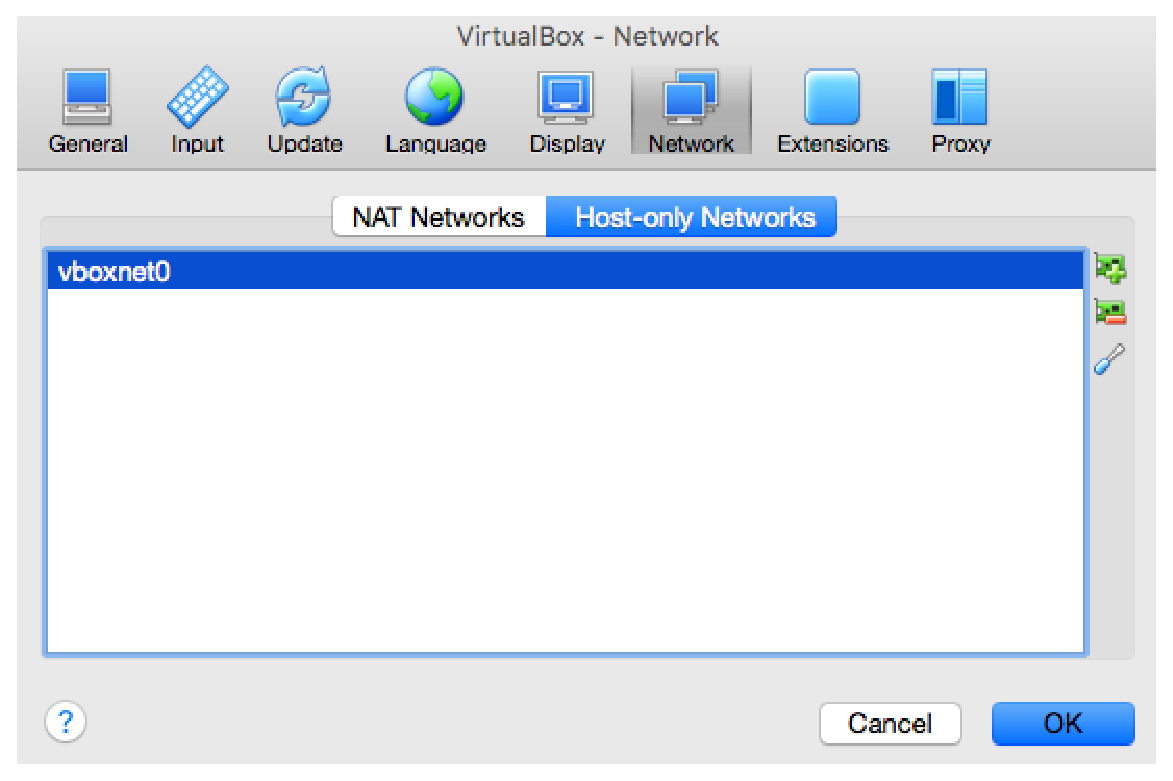
\includegraphics[scale=0.65]{figures/virtualbox-host-only-network}
    \caption{Creating a New Host-Only Network in VirtualBox}
    \label{fig:virtualbox-host-only-network}
\end{figure}

\begin{figure}[ht]
    \centering
    
\includegraphics[scale=0.65]{figures/vm-network-adapter}
    \caption{Second Network Adapter Configuration}
    \label{fig:vm-network-adapter}
\end{figure}

\clearpage

Figure \ref{fig:vm-network-manager} shows what the system network manager displays about the \glspl{vm} network configurations.

\begin{figure}[ht]
    \centering
    
\includegraphics[scale=0.65]{figures/vm-network-manager}
    \caption{System Network Manager Displaying Two Network Interfaces}
    \label{fig:vm-network-manager}
\end{figure}

But even with connectivity achieved between the two \glspl{vm} through the host-only network, random IP addresses were assigned at each boot time. In fact, just like VMWare, VirtualBox comes out with a default DHCP server. To avoid further configuration changes within the \gls{json} configuration file, I just had to set static IP addresses so that their IP addresses would be persistent throughout reboots.

Finally, Figure \ref{fig:network-configuration} shows an overview of the network configuration. Each \gls{vm} has two network adapters, one for internet access which is directly connected to the system's network via NAT protocol, whereas the other is devoted to the virtual and private host-only network between the two \glspl{vm}.

\vspace{0.5cm}

\begin{figure}[ht]
    \centering
    \includegraphics[scale=0.45]{figures/network-configuration}
    \caption{Network Configuration Overview}
    \label{fig:network-configuration}
\end{figure}

\clearpage

\subsection{Running LAVA}
\label{sec:lava-example}

\subsubsection{JSON File Configuration}

Once the environment configuration done, I only had to set the correct static IP addresses in the \gls{json} configuration file to make \gls{lava} run. As previously stated, \gls{lava} uses a \gls{json} configuration file to define its execution, and keep precious information. Listing \ref{lst:json-config-file} shows the format for the \gls{lava} \gls{json} configuration file.

\vspace{0.5cm}

\lstinputlisting
    [
        caption=\gls{json} Configuration File for Lava on the File Program,
        label=lst:json-config-file
    ]
    {listings/json-config-file.json}
    
Notice the main information fields:

\begin{labeling}{testinghost}
    \item[\emph{buildhost}] The buildhost corresponds to the IP address of the 32-bit \gls{vm} hosting the compilation of the base program to be injected with bugs.
    \item[\emph{testinghost}] The testinghost corresponds as well to the IP address of the 32-bit machine which is responsible for assessing the injected bugs by testing the modified program with the bugs triggering inputs.
    \item[\emph{pandahost}] The dynamic taint analysis and metrics compilation to look for \glspl{dua} and \glspl{atp} are realized thanks to the dynamic analysis platform PANDA's taint system. The pandahost henceforth refers to the IP address of the 64-bit machine which is responsible for the dynamic taint analysis of the base program.
    \item[\emph{lava}] This field corresponds to the path of the \gls{lava} software on the system.
    \item[\emph{qemu}] This field corresponds to the path of the QEMU software on the system. Notice that we need QEMU because PANDA is based on it. In a few words, QEMU is a virtualized environment in which PANDA records the executions of the tainted program.
    \item[\emph{tarfile}] This is the path to the base program tarball to be injected with bugs. In our file example on Listing \ref{lst:json-config-file}, it is the \emph{file} program.
    \item[\emph{dbhost}] The dbhost field refers to the IP address of the 32-bit \gls{vm} which hosts the \gls{lava}'s POSTGRES database. A lot of information is stored in it, and we will see how we make use of that database to retrieve the \glspl{dua} and \glspl{atp} locations in the source code.
\end{labeling}

The other fields, like \emph{max\_liveness}, \emph{max\_cardinality}, and \emph{max\_tcn} are used to set parameters for the execution of \gls{lava}. It directly influences the way the taint-based analysis is processed by setting threshold values for the liveness and \gls{tcn} computation.

\subsection{LAVA Demo -- Execution Overview}

A typical execution of \gls{lava} is composed of four main steps (Figure \ref{fig:lava-process}):

\begin{enumerate}
    \item Instrument the base program source code with taint queries and compile it. The CLANG compiler takes care of that step by adding code into the base program. This added code queries PANDA to make a taint analysis on the source locations pointed by the instrumentation
    \item Run the dynamic taint analysis with PANDA, which is composed of two subroutines:
        \begin{enumerate}
            \item Record executions of the instrumented program
            \item Replay those executions with taint propagation
        \end{enumerate}
    \item Analyze the taint analysis results and compute the liveness and \gls{tcn} metrics in order to identify \glspl{dua} and \gls{atp}
    \item Finally, inject the bugs and assess the injection success by testing the bugs with the corresponding triggering inputs
\end{enumerate}

\begin{figure}[ht]
    \centering
    \includegraphics[scale=0.35]{figures/lava-process}
    \caption{LAVA Implementation Architecture \cite{dolan2016lava}}
    \label{fig:lava-process}
\end{figure}

The LAVA team designed a little demo to showcase their software use on the \emph{file} program. Figure \ref{fig:lava-demo} shows the output of that demo when running \gls{lava} on the file program.

\begin{figure}[ht]
    \centering
    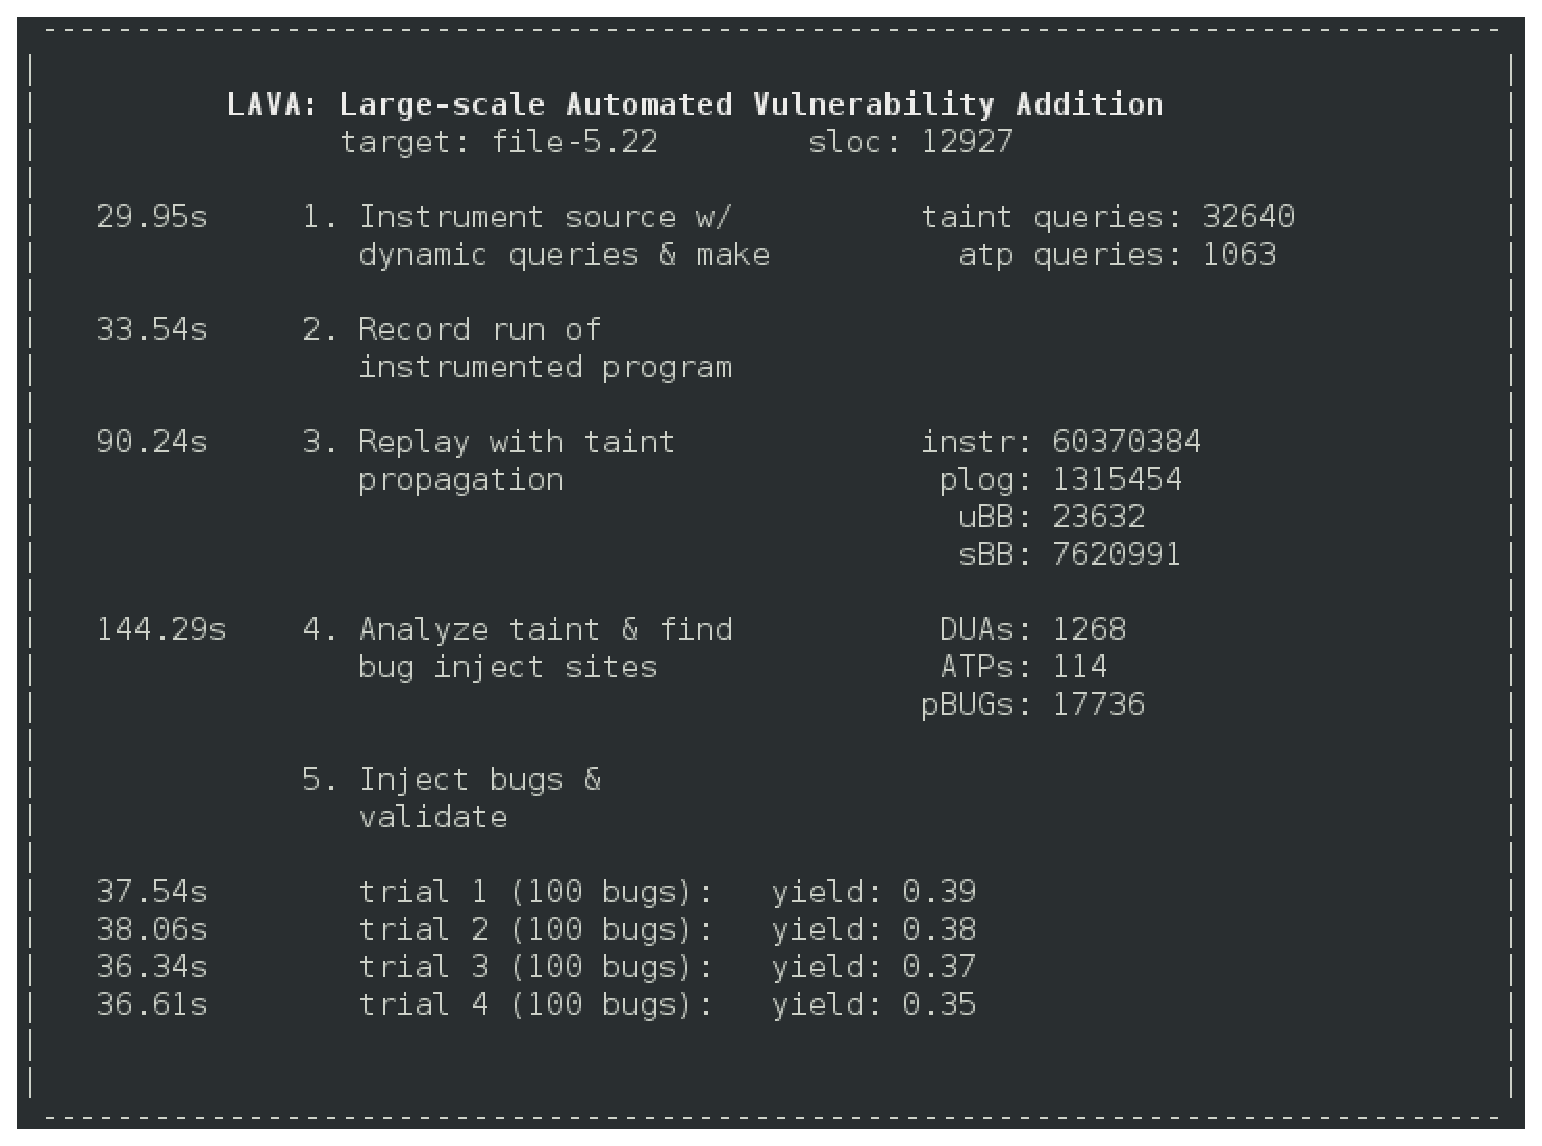
\includegraphics[scale=0.5]{figures/lava-demo}
    \caption{LAVA Demo Running on the File Program}
    \label{fig:lava-demo}
\end{figure}

Notice that the number of potential bugs (\emph{pBUGs}) is quite high for a small program like \emph{file} (\~10k \glspl{sloc}). The number of potential bugs is almost proportional with the product of the number of \glspl{dua} and \glspl{atp}. The yield value refers to the number of bugs that were successfully injected during step 5. The asymptotic behavior is a 40\% yield which means that on average 40 bugs out of 100 are successfully injected.

\subsection{Making Use of LAVA information}

To achieve our aims, we do not need to go through all the execution steps of \gls{lava}. In fact, our only interest is in the identification of the \glspl{dua} and \glspl{atp}.

Fortunately for us, all the information about the taint analysis is stored in the POSTGRES database. In order to make use of this precious intelligence, I decided to design an SQL request that would allow us to retrieve the essential information we need to guide us through our manual vulnerability seeding.

As previously stated, the \gls{lava} `formula' for a bug is the pair combination of a \gls{dua} and an \gls{atp}. This `formula' can be retrieved in the way \gls{lava} team designed their POSTGRES database which is composed of a table \emph{bug} with three fields: a bug identifier, a \gls{dua} identifier, and an \gls{atp} identifier. Two more tables \emph{dua} and \emph{atp} contain specific information about the \glspl{dua} and \glspl{atp} such as their location in the source code.

This information is exactly what we need in order to know where to look in the source code for manually seeding vulnerabilities. Therefore, I designed the following SQL request providing in Listing \ref{lst:sql-request}, which output can be found in Figure \ref{fig:sql-output}.

\vspace{0.5cm}

\lstinputlisting
    [
        language=SQL,
        caption=SQL Request,
        label=lst:sql-request
    ]
    {listings/everything.sql}

\begin{figure}[ht]
    \centering
    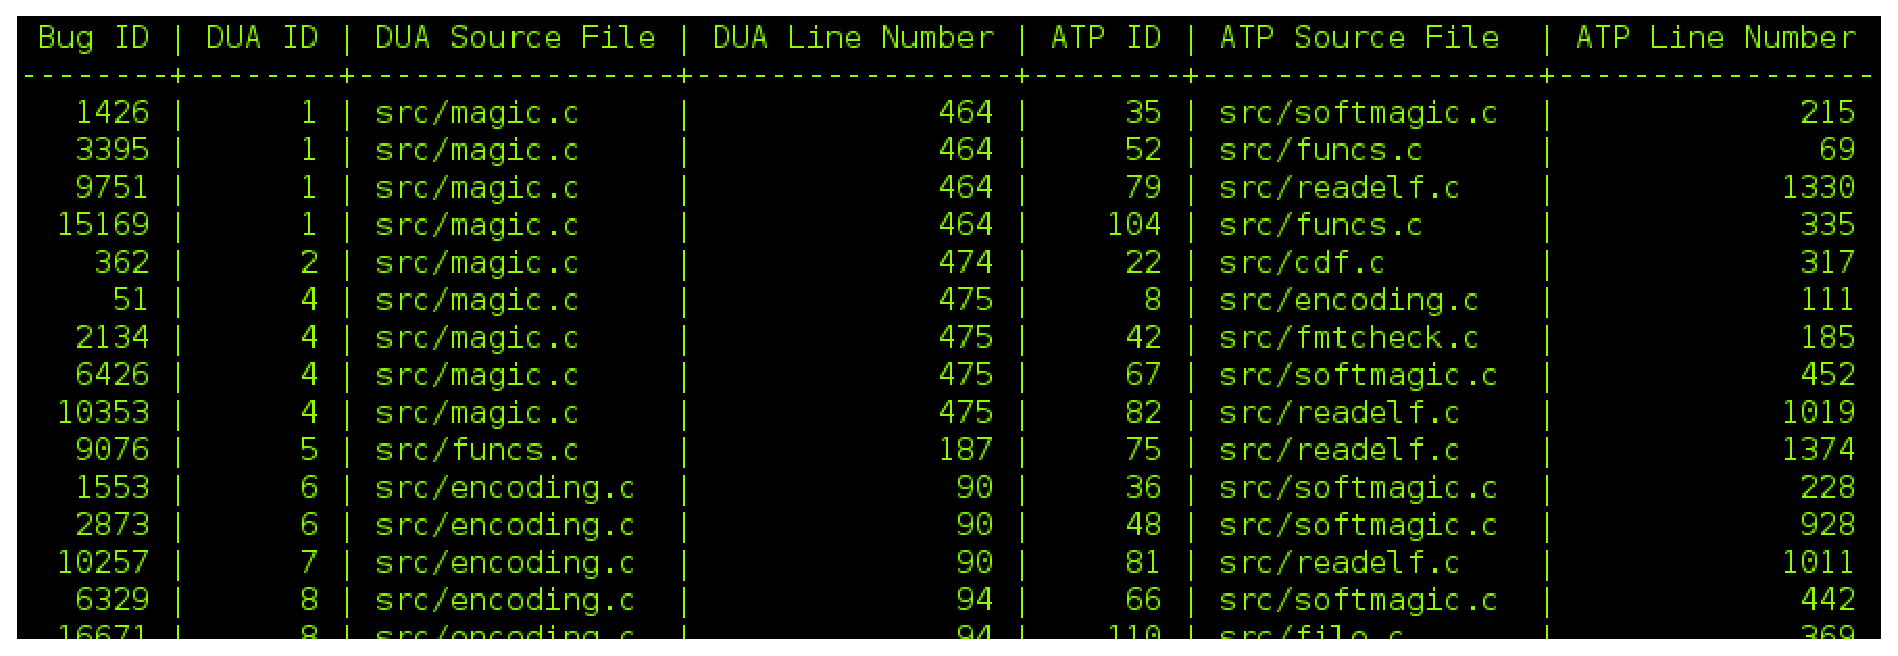
\includegraphics[scale=0.5]{figures/sql-output}
    \caption{Output of the SQL request (Listing \ref{lst:sql-request})}
    \label{fig:sql-output}
\end{figure}

\subsection{Running LAVA on the \emph{hping} Program}

So far, I did not have the time to go further than this step. According to my work schedule, I managed to configure a \gls{lava} environment, I successfully ran the software on the provided example \emph{file} program, and I got familiar with the LAVA implementation architecture to the point I was able to design a solution in order to retrieve the \glspl{dua} and \glspl{atp} locations in the source code.

The next step is to run it on a potential futur test case, starting with a small example like the Linux \emph{hping} program. However, I am still working on some compilation issues encountered with the CLANG compiler, and therefore this step should be considered in progress.